\renewcommand\labelenumi{(\roman{enumi})}
\renewcommand\theenumi\labelenumi

\chapter{Introduction}
\label{chapterIntro}
\chaptermark{Introduction}

The current society is facing a challenge in order to mitigate the effects of the climate change. With the objective of keeping global temperature rise below 2 degrees Celsius as stated in the Paris Agreement XXXX, the whole energy system is called to an action: transform a mainly fossil-based electricity generation scenario to one that is carbon-neutral, mainly based on renewables energy sources (RES). The challenge is even greater, since it is expected that the electricity consumption will increase from a 20\% to 40\% by 2050, according to \cite{IRENA2018}. This can be observed in Figure \ref{fig:scenarios}, where the scenario by 2050 expects the 85\% of the electricity supply to be covered by renewables. This chapter aims to provide an overview of the current state of the electricity system and their agents, so as to highlight the main shortcomings, challenges and opportunities for the implementation of the energy transition roadmap. The following pages cover the regulation related to DSOs and smart grids, the technical aspects of DERs and ICT technologies, the role of demand-side and end-user's awareness, and lastly the role of new business agents and services that can help DSOs to become key agents in the development of smart grids. 


\begin{figure}[]
	\centering 
	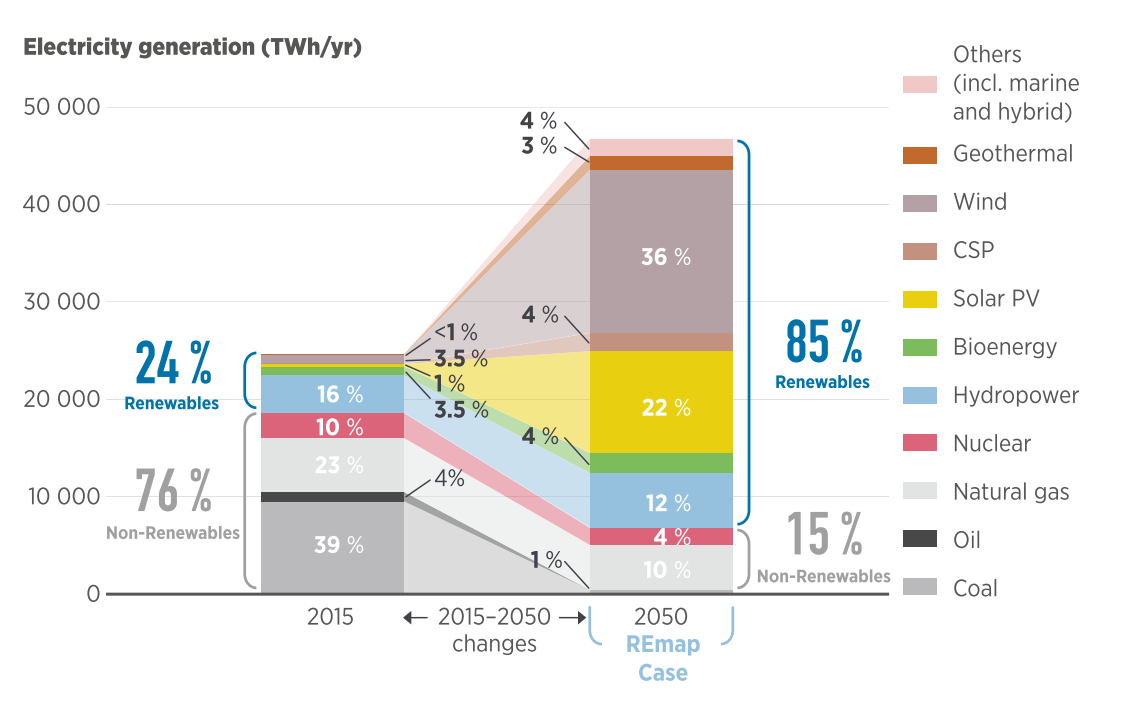
\includegraphics[width=0.8\columnwidth ]{ChapterIntro/Figures/irena_scenarios.png}
	   %\vspace*{-8cm}
		\caption{Renewable Energy Sources penetration scenario. Extracted from \cite{IRENA2018}}  
		\label{fig:scenarios}
\end{figure}


\section{Smart Grids. The evolution of the electrical network}

%\subsection{Electricity network}
The physical infrastructure of the electricity network is composed by generators, transmission network, distribution network and end-users or consumers, as shown in Figure \ref{fig:ree}. 

\begin{figure}[h]
	\centering 
	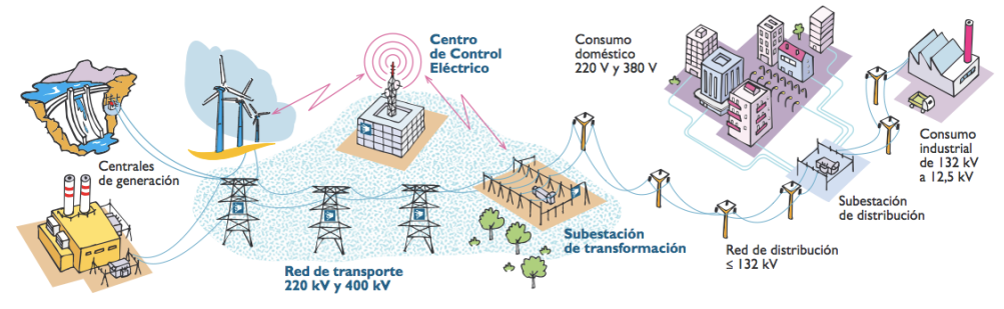
\includegraphics[width=0.8\columnwidth ]{ChapterIntro/Figures/ree.png}
	   %\vspace*{-8cm}
		\caption{Electricity network scheme. Extracted from XXX}  
		\label{fig:ree}
\end{figure}

Generators are the main agents feeding the grid downstream. Large generators can produce a range from 6 kW to 20 kV [XXX], to then increase the voltage up to 200 kV in order to connect to the high voltage (HV) tramission lines. The transmission network is the responsible for the electricity transportation over long distances, and it is done at HV level. By doing this, the transmission losses are lower while using a cheaper infrastructure. The tranmission network voltage level usually ranges from 200 kV to 1000 kV [XXX], and both generators and HV-MV transformers are the main elements connected to it. Due to their critical position in the system, connecting generation and consumption sides, transmission grids are meshed to avoid collapsing when there is any failure in on of the lines. On top of that, this layout allows the distribution of the loads through different tramission lines with the objective of reducing losses and avoiding congestions. Transmission networks are operated by the so-called Transmission System Operators (TSO). Similarly, distribution networks are responsible for the energy distribution and transportation for shorter distances. One could consider a distribution grid when its voltage levels are either medium-voltage (MV) and low-voltage (LV). By definition, the voltage levels considered for distribution networks are: 132 kV, 66 kV, 45 kV, 30 kV, 20 kV, 10 kV, 6 kV, 3 kV, 1 kV, 400 V and 230 V [xxxx]. 

Differently as seen in the transmission system, the assets connected at distribution level are mainly loads ranging from industrial loads, connected at MV, to residential loads, most usually connected at the LV level. However, generation units can also be connected  at the distribution level, usually only considering renewable sources. The configuration layout of distribution networks is commonly not redundant, meaning that they do not usually use meshed configurations. As a result, these networks are not as redundant as the transmission system. Hence, this could lead to problems when DERs are connected to MV or LV connection points, leading to congestions  in distribution networks that were not expected when the network was implemented. Distribution networks are managed by Distribution System Operators (DSO), who connect consumers, install electricity meters and communicate the end-user consumption to energy suppliers or retailers [XXX]. 


\begin{figure}[h]
	\centering 
	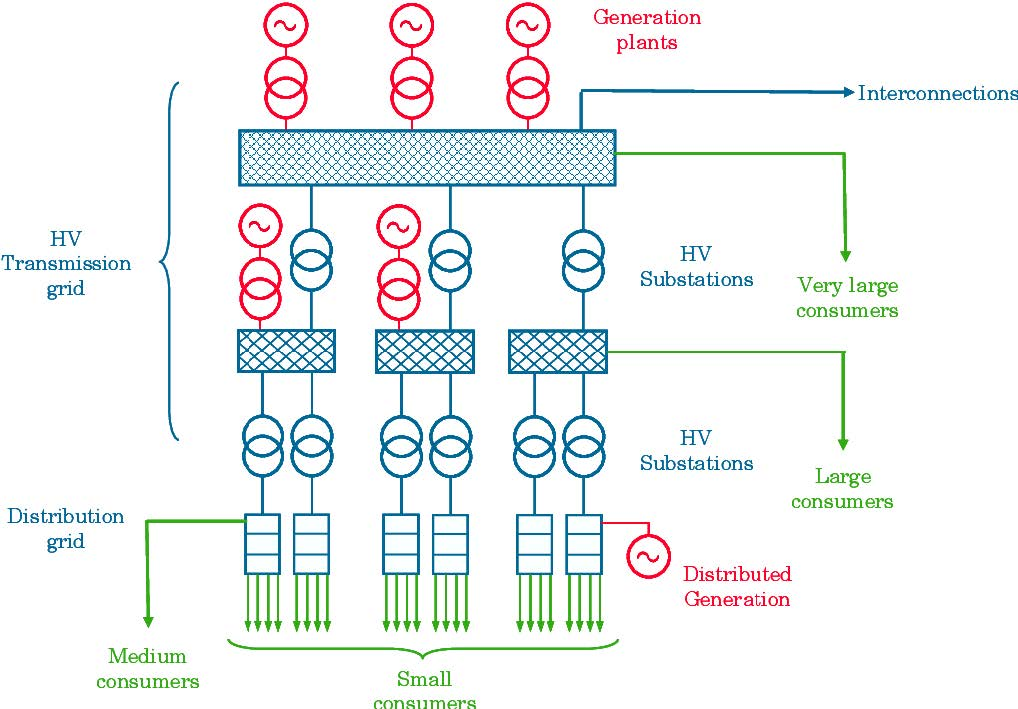
\includegraphics[width=0.8\columnwidth ]{ChapterIntro/Figures/ELECTRICITY_SYSTEM.jpg}
	   %\vspace*{-8cm}
		\caption{Electricity network scheme. Extracted from XXX}  
		\label{fig:ree}
\end{figure}

%\subsection{Smart Grids}

Despite the scenarios where renewables are the main source for electricity production, it is a fact that large power plants placements are more difficult to find XXX, leading to newer technologies to allocate renewable sources in places where a larger power output can be obtained, and less concern by end-users in terms of environmental and visual impact of them, such as off-shore wind turbines XXXX, connected to the transmission network. At the same time, as electricity demand on grids increased due to the electrification of appliances, distribution system operators (DSOs) started to face congestions in their networks, and hence utilities started to find solutions for managing these peak loads, usually located in specific time periods.  This combined to the implementation of smart meters so utilities could encourage customers to switch consumption from peak to non-peak hours, and the need for monitoring and controlling the operation of the distribution network enhanced the development of smart grids. Traditionally, electric power systems have been centralizsed structures organized into generation, transmission and distribution, placing end-users and the endpoint of the supply chain. This was an unidirectional structure where electricity generated by large power plants was transported by means of transmission and distribution networks, to be delivered to end-users. Despite, the emergence of the social awareness of the environmental impact of the end-users consumption, the increase of the electricity prices, as well as the emergence of the so-called distributed energy resources (DERs), such as small-scale PV installations (mainly rooftop), storage systems, electric vehicles (EVs) and smart home appliances are transforming the end-users into active participants in the power system. The increasing penetration of these decentralized resources, as well as the emergence of new market agents like prosumers, aggregators and active consumers, are pushing the electricity system to include innovation in their business models, creating the paradigm of smart grids (Figure \ref{fig:IRENA-DSO}). 

\begin{figure}[h]
	\centering 
	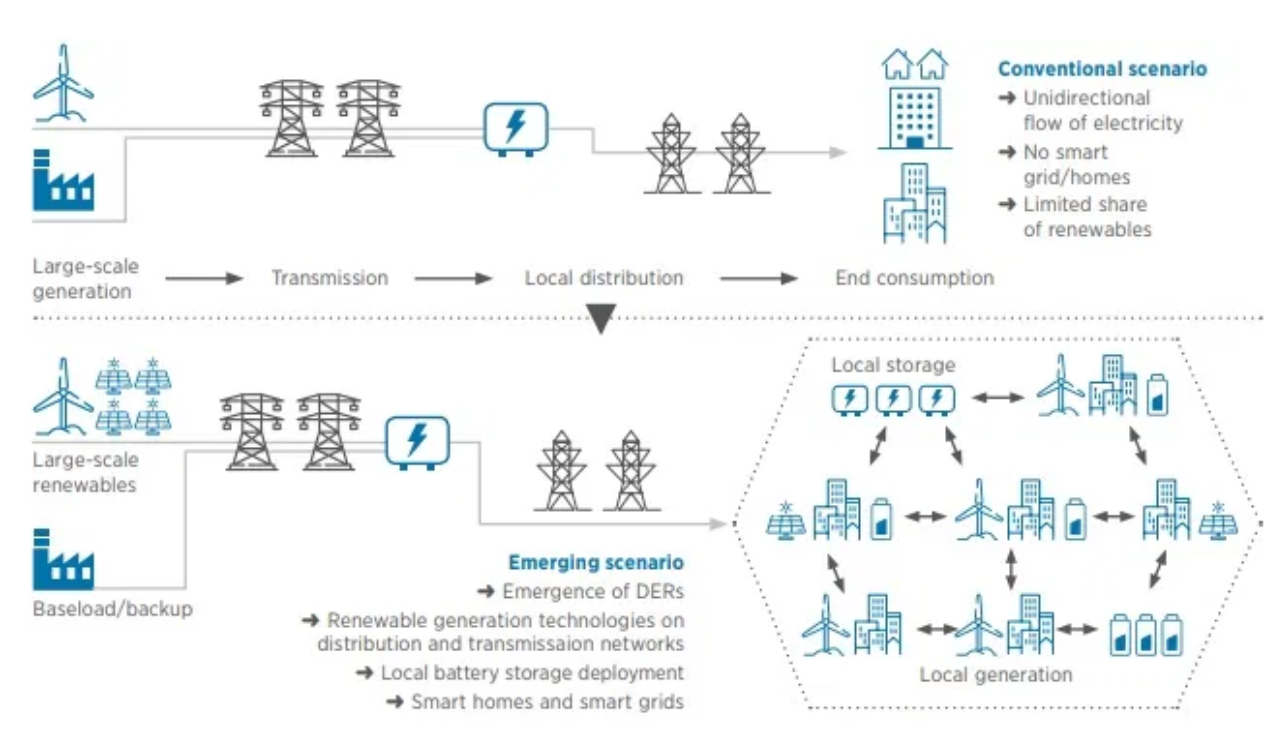
\includegraphics[width=0.9\columnwidth ]{ChapterIntro/Figures/Irena-DSO-1.png}
	   %\vspace*{-8cm}
		\caption{Conventional scenario vs Smart Grids. Extracted from \cite{IRENA2018}}  
		\label{fig:IRENA-DSO}
\end{figure}


According to \cite{EuropeanParliamentSG}, smart grids can be defined as:

\begin{tcolorbox}
\textit{"an electricity network that can integrate in a cost efficient manner the behaviour and actions of all users connected to it, including generators, consumers and those that both generate and consume, in order to ensure an economically efficient and sustainable power system with low losses and high levels of quality, security of supply and safety".} 
\end{tcolorbox}

However, it is not only in terms of technological innovation to fulfill the electricity transition roadmap. Changing the regulatory framework mainly for DSOs to adapt the current regulation for the operation of the distribution network to the new challenges placed by DERs is a key factor for the success of the energy transition.

With the liberalisation of the electricity markets all over Europe, due to the promotion of directives such as the ones in the First, Second and Third Energy packages (respectively: XXXX) to create a more robust internal market XXXX, grid planning faced problems related to generation forecast. Because at that point the generation at the HV side of the grid was not 100$\%$ planned anymore. However, the network overcame the problem establishing rules where these new agents must inform of their operations a centralised organisation in order to maintain the balance of the system, and creating a markets-system where TSOs upload their needs and generators their offers. 

Nowadays the EU is promoting another change in the structure of the electricity market, imposed by the need to decarbonise the energy sector by 2050 and the willingness to empower the citizen changing its role from pure consumer to a new agent in the market [27]. This is mainly going to be done by promoting the integration of DERs in the distribution grid which supposes an entirely new approach to the grid management. Challenges like reverse power flows and an increase of voltages near the point of coupling, among others, will arise. This structural change of the electricity system has been changing habits in the sector for some years now, and with 
these new ways to proceed challenges have arisen, from [30] the main changes can be classified as:

\begin{enumerate}
\item With the liberalization of the generation, system operators are less capable of limiting
connections of new generation assets which can drive the grid, at some locations, to its
limits.
\item Formerly traditional PGMs location was determined considering the interests of the system
operator and the constraints related to the construction of such large power plants.
Nowadays, the location of new RES power plants is instead related to energy source availability.
\item RES generation tends to connect at distribution level instead of transmission level where
all the main PGMs were connected.
\item Democratization of generation assets which, other than the new cases stated above, can
transform traditional passive-customers to active customers and thus increase the variability
of the demand.

\end{enumerate}

These four changes in the power system structure can and will be an improvement in terms of clean generation, increased energy efficiency, customer empowerment, and grid reliability, among others. However, the truth is that nowadays most of the European grids are far from being ready to face such challenging opportunities and these new approaches are also making arise new problematic, and not-so-new ones, that can be divided into two main groups: 
\begin{enumerate}
\item Generation and load balancing: If there is no balance between generation and demand, the frequency of the system starts to deviate from the nominal value; this may be a problem for some electric/electronic loads. However, the main concern arises when large generators are synchronous machines. In an intense frequency deviation event some generators may trip from the grid, causing even a harder frequency deviation. This domino-like problematic is called cascade tripping and can lead to a local or even "global" system blackout. This problematic has been a concern for the system since its beginnings because the load forecast is not always accurate. However, large PGMs can be mandatorily disconnected from the grid for safety purposes [30]. Then, the challenge increased with the liberalization of the generation market. Nowadays, with the introduction of DERs and the empowerment of the user via demand-modulation strategies, the future forecast of generation and demand is expected to be more challenging than ever.

\item Distribution grid congestion: Grid congestion, mainly at TSO level but also at DSO level,has always existed. However, due to the traditional operation of the grid, the fit-and forget approach consisting of investing in expanding the infrastructure was the most costefficient approach at the distribution level. With the uncontrolled connection, in terms of number but also location and characteristics, of new DER assets to medium and low voltage grids, a new grid structure may be needed from the fit-and-forget perspective. However, this does not seem either rational nor cost-effective viable, and instead, these new congestion challenges will need to be addressed from an active (real-time) management approach.
\end{enumerate}


\section{Regulation framework and new agents in the energy transition}
For the last 15 years or so, climate change, global warming, and generally a more rational approach to production and consumption habits have been an increasing concern for societies with a firmly established welfare state. Related to this new approach to the production system, from the first-day electricity markets have been the target of criticism due to their massive contribution to the emission of greenhouse effect gases XXXX. Within the European energy policy context, the chosen way to carry out this reduction of emissions by the energy sector is enhancing a higher penetration of DERs (particularly RESs) in distribution networks. This positioning, while has multiple potential benefits for the grid and its agents, also sets out new challenges.
All the perks and disadvantages of a higher share of DERs need to be adequately regulated in order to keep secure the functioning and operation of the grid. It also has to be noted that inside the EU energy policies, the environmental concern is nowadays
one of the main drivers. However, there are also other key objectives to achieve, which in some cases will present synergies, but in other cases, could collide among them. 

From another perspective, "not-so-concerned-with-the-environment" countries due to major problems, are also looking to a transition in the generation model. In this case, many factors can drive the decision. However, an important one may be the economic easiness of developing a DG network involving smaller stakeholders instead of making the needed substantial public investments in developing a traditional schemed grid [55].

The creation of the Winter Package the year 2016, also known as Clean Energy Package for all Europeans, started after the European Commission had evaluated the performance of the Third Energy Package established in 2009.  After assessing the outcomes of the previous energy packages, the objectives starting back then could be grouped in three, as follows: 
\begin{enumerate}
\item Adapting to the decentralization of the power system. 
\item Empowering cuustomers and citizens. 
\item Ensuring the internal market level playing field. 
\end{enumerate}

About the CEP itself, first it has to be knownthat it is a set of regulations and directives published in June 2019 to promote the energy transition started with the Third Energy Package back in 2009. Among the CEP regulations and directives, the ones that address the electric sector are the e-Directive (EC 2019/944; [14]) and the e-Regulation (EC 2019/943; [15]), whose subject matter and scope is centred in \textit{"setting the basis for an efficient achievement of the objectives of the Energy Union and in particular the climate and energy framework for 2030"} (e-Regulation), \textit{"via the creation of common rules for all the assets connected to the power system, with a view to creating truly integrated, competitive, consumer-centred, flexible, fair and transparent electricity markets in the Union"} (e-Directive). The e-Directive and e-Regulation are mainly focused towards the creation of market models to
promote the energy transition. In terms of market design there is a group of markets, flexibility markets, that can be crucial to promote the widespread of new agents and technologies [67].


\section{Flexibility as a service for the energy transition}
Power system flexibility will play a key role in the energy transition and the next generation electric grid, and some of the main outcomes of implementing flexibility are the possibility to replace fossil fuel generators with clean and renewable energy sources; increase reliability and resilience against disruptive events; improve performance and reduce cost of new and existing assets and achieve the scenario where a low carbon economy is possible. 

In the traditional organization of the power grid, large PGMs were forced to be able to provide flexibility. Some of these requirements for large generators are still considered in the new regulation under the Clean Energy Package and Grid Codes. However, most of the requisites are not mandatory for smaller PGMs, and in some MSs legislation, RES power parks that fit in the large PGMs definition are excluded from the fulfillment of these requirements. With the new paradigm decreasing the number of synchronous PMGs and more difficulties than ever to forecast demand and generation, the large PGMs remaining may not be able to handle the flexibility required to keep the grid working correctly. This will
suppose an increased need for flexibility [35]. Also, the penetration of DG into the MV and LV grid will suppose some challenges, as seen in Section 3.3, which will need to be addressed by the DSOs via active grid management. Finally, the provision of local flexibility will help not only to secure the grid operation but also to improve grid efficiency efficiency during normal operation time [18].
For these reasons, improved flexibility markets are being recognized in the e-Directive as a pillar to support the safer and more efficient use of the existing grids, and to enhance the HC of distribution feeders. Since the scope of this work is to research those regulations that enhance RESs penetration while guaranteeing safe operation of the power grid, it is interesting to study how flexibility markets could be designed in order to promote DERs participation.

In general terms, flexibility can be defined as "the ability of a power system to reliably and cost-effectively manage the variability and uncertainty of demand and supply accross all relevant timescales", defined by the International Smart Grid Action Network (ISGAN) \cite{Hillberg2019}. 
According to the same institution, flexibility will enable all stakeholder and elements of the grid considering generators, consumers/end-users, storage and infrastructure to be active participants in the energy system, also enabling the cost-efficient development of RES and more resilient power systems. 
Traditionally, these variations from the demand side have been overcome by means of fuel-based flexible generators such as carbon and gas turbine; and pumped hydro power plants. Those changes on the demand-side where mainly from changes in the load consumption based on consumer behavior. 

However, since there is an increase on DERs, the consumer behavior patterns have been broadly studied XXXX, showing that the electricity consumption is focused at specific time periods, such as noon and in the evening. With the implementation of DERs and the increase of the electricity consumption, there is a possibility to include flexibility in power systems by achieving the paradigm where consumption follows the generation curve only partially. That could lead to implement flexibility in the demand-side by shifting the consumption of some assets or the production of some small scale generators or storage systems to other time periods, as seen in Figure \ref{fig:load_shifting}. 

\begin{figure}[h]
	\centering 
	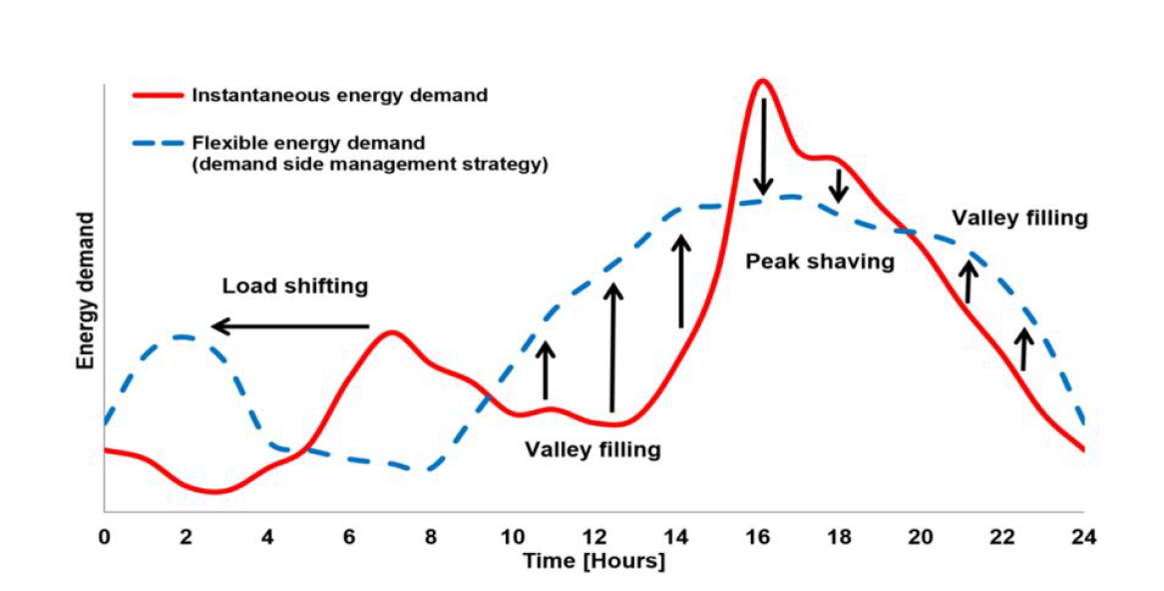
\includegraphics[width=0.8\columnwidth ]{ChapterIntro/Figures/flex_load_shifting.png}
	   %\vspace*{-8cm}
		\caption{Flexibility effects on electricity consumption. Extracted from \cite{Hillberg2019}}  
		\label{fig:load_shifting}
\end{figure}


\section{Sustainability of smart grids and DERs}
The increase of renewable generation has provided many benefits in the road towards a decarbonized power system. However, in the past years, social concerns about the environmental impact of renewable technologies have arisen \cite{Temper2020}, with more than 3000 environmental conflicts based on renewable energy-related projects. These problems are based on the fact that these projects do not take into consideration neither the acceptance of the population living close to the renewable energy plant location, nor the consequences of having the power plant, such as the reduction of agriculture fields or the impact on the land prices. 

Hence, the decentralization of the renewable generation with the appearance of DERs has a large potential to succeed in the energy transition roadmap. However, sustainability must be taken into consideration in each and every step, even in local energy communities and DERs \cite{AMPONSAH2014461}. Some of the current methodologies for calculating the environmental impact of renewable energy technologies assume that the carbon footprint of renewable sources is zero, because they only consider the $CO_2$ emission factor under the operation phase \cite{IRENA2020}. However, there is a non-negligible carbon footprint or other environmental impacts such as water usage and polution and ozone contribution that must be considered. Furthermore, when developing smart grids and renewable energy sources and energy transition policies, a previous analysis should be performed in order to understand the current installed capacity in the country, in order to lower the environmental impact by implementing such technologies.

Technologies and methodologies such as circular economy, second-life possibilities and life-cycle assessment are key to check the viability of renewable energy projects and smart grids implementation. Life-cycle assessment (LCA) can be a powerful a tool for assessing environmental impacts of renewable energy sources, so as to assess the environmental impact based on indicators of renewable energy technologies and smart grids throughout the entire lifecyle.
 


%\newpage 
\section{Objectives and scope}
Several past and recent works in the literature have dealt with the development of smart grids and defining local electricity markets for enhancing the energy transition. The majority of these studies consider flexibility as a known signal, assuming a perfect forecast and a direct control of the flexible assets, as a way of simplifying the operation of the local flexibility markets. Furthermore, they assume that both the aggregator and the DSO share information regarding the flexible assets or the network layout. The fact is that, in reality, and according to the current regulation, they must be different entities, considering 

The main research question that this thesis aims to answer is the following one:

\begin{tcolorbox}
What are the possibilities to develop and activate flexibility in distribution networks, by engaging demand-side and ensuring that the sustainability goals are taken into consideration? 
\end{tcolorbox}

This can be considered a broad question, and hence the knowledge barriers should be found in order to establish the baseline for the PhD research. This manuscript aims to answer this question focusing on the role of the demand side and their flexible assets and what the benefits and consequences would be for distribution networks, managed by DSOs. Figure \ref{fig:objectives} provides an overview of the system under study, considering the demand-side by means of prosumers and flexible assets; the aggregator as the entity that collects all the available flexibility and provides this service to the DSO by controlling the end-user's assets; the DSO as the main client of this flexibility; the electricity market to understand which role plays the flexibility in a market-environment; and lastly the environment, to assess the global warming potential and other environmental impacts that flexibility could reduce or increase. Based on the previous discussion, more specific objectives can be outlined in order to set the basis for the research developed in this thesis. The objective of the thesis are outlined below: 

\begin{tcolorbox}
\begin{enumerate}
\item What are the possible market schemes to integrate DERs and demand-side management, while at the same time ensuring that network operators can benefit from these services?  
\item How can flexibility be defined and modeled, based on the final users providing and using this flexibility, as well as the time horizon purposes? 
\item How can flexibility be forecast, from the aggregator point of view, with very limited amount of data available, in a fast and reliable approach so as to know in advance the flexibility available in the portfolio, in order to provide flexibility to DSOs for operation purposes?
\item How can this flexibility help DSOs to mitigate or avoid congestions in MV networks, and how can this flexibility request be calculated so as to be economically better than investing in network expansion or hosting capacity?
\item How this scenario of flexibility provision can be environmentally assessed, so as to know if these approaches can be included in each and every country? Should the current installed capacity and generation portfolio be taken into account before the deployment of flexibility services in smart grids?
\end{enumerate}
\end{tcolorbox}

A conceptual overview of the different objectives outlined above is shown in Figure \ref{fig:objectives}, which can be also understood and the steps taken in this thesis. 

\begin{figure}[h]
	\centering 
	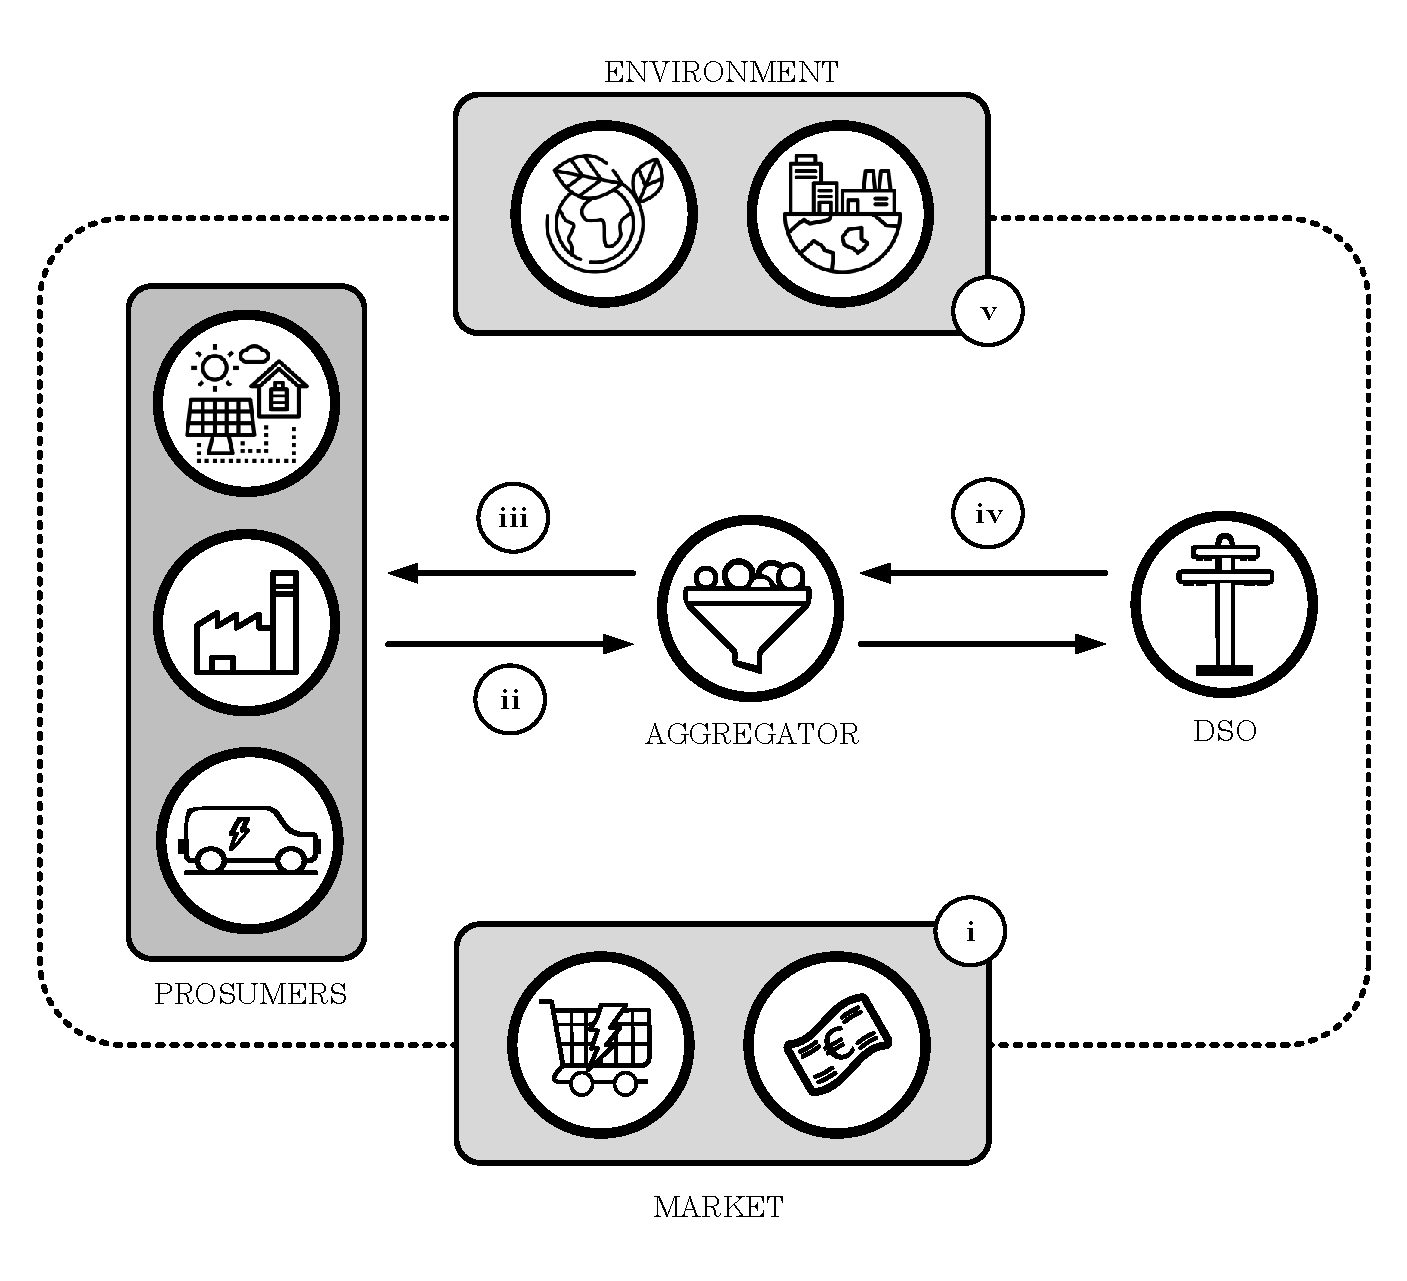
\includegraphics[width=0.8\columnwidth ]{ChapterIntro/Figures/objectives_figure_2.pdf}
	   %\vspace*{-8cm}
		\caption{Overview of the thesis objectives}  
		\label{fig:objectives}
\end{figure}

More specifically, each of the questions and objectives can be detailed and related to each of the chapters of this manuscript. 
\


%\newpage 
\section{Thesis related work and activities}
This section provides a summary of the work and the relevant activities that the author has participated in during the developlment of the thesis presented in this manuscpript. 
 	
Doctoral activities started in June 2017 with the collaboration on behalf of the EMPOWER \textit{Local electricity retail markets for prosumer smart grid power services } Project (Grant Agreement No. 646476). This work consisted on a review of the current state of the art in terms of Life Cycle Assessment Methodology in the field of smart grids, the understanding of how this methodology can be implemented in power systems and renewable energy technologies and the assessment of the environmental impact of the pilot-sites implemented throughout the project. This research resulted in a presentation in the General Assembly of the H2020 Project [P-C1] and the technical report [TR-2]. The research on the environmental assessment of ICT and Smart grids continued in the H2020 Project INVADE \textit{Integrated electric vehicles and batteries to empower distributed and centralised storage in distribution grids} (Grant Agreement No. 731148), in years  2018 and 2019, with the assessment of the environmental impact of electricity generation and the possibility of including flexibility to lower the environmental impact of electricity production in the INVADE pilot-sites. This research was performed in collaboration with the Finnish research center VTT, NTNU, Elaad and eSmart resulted in the journal publication [J1], a conference proceeding [C2], and technical reports [TR3], [TR5]. Dissemination events for the exploitation of the results took place in years 2019 and 2020, [P-C5] and [P-C11]. 

Since the main objective of the thesis is how new local markets and new service can help the deployment of smart grids, a thorough review of the state-of-the-art on local electricity market was done as a starting point of the doctoral research in 2018. This research was mainly focused on describing the basics on power systems and market mechanisms, as well as a literature review on local and micro-markets. As a result of that, a technical report was developed [TR1], and two book chapters were published by Wiley ([BC1],[BC2]).  The evolution of this state-of-the-art review, combined with the collaboration with colleagues at CITCEA-UPC and other research centers and companies such as EYPESA and Smart Innovation Norway or on behalf the INVADE Project led to several outcomes covering from technical reports [TR4], journal articles [J4] adnd [J5]; conference papers [C1], [C3] and [C4]; and presentations in local and international events [P-C3] and [P-C4].  

The evolution and implementation of smart grids based on data-driven approaches has been of interest of the author, and combined with collaboration with other universities as KU Leuven, DTU and KTH Stockholm on behalf of EIT InnoEnergy, resulted in [P-C6], [P-C10] and [P-C14]. 

%Escriure BD4OPEM aquí 
Year 2020 started with the kick-off the BD4OPEM H2020 Project \textit{Big Data for Open Innovation Energy Marketplace} (Grant Agreement No. 872525), with the participation of 12 partners from 8 different countries, and 5 pilot-sites. The research consisted on the development of algorithms for flexibility forecast and distribution network congestion management based on optimization techniques and flexibility provision. This work was combined with the Technical University of Denmark (DTU) under the external stay of the author, and in collaboration with other research centers and companies such as JSI and ICOM. This work resulted in a technical report [TR6], two dissemination events [PC-12], [PC-15], and three journal publications under review or preparation [J2], [J3] and [J6].  

The international placement took place from March 2020 until April 2021, at the Electricity Markets (ELMA), DTU, Kongens Lyngby, Denmark. The topic was aggregated flexibility forecast based on probabilistic forecast techniques. It resulted in a journal paper [J2], and the database publication [DB1]. During this period, the author has collaborated with KU Leuven in the core of the Data Science Working Group, with the aim of improving the knowledge of undergraduate students in the field of data science in the energy sector. This resulted in the publications [J7] and [J8]. 

Since the author and the research center where the thesis was involved has a flair for knowledge transfer and higher and professional education, the author has collaborated with other entities and other researchers, resulting in the respective outcomes, which are not included in the thesis manuscript. This is the case of the collaboration with EIT InnoEnergy. This European institution has as a main core activity the connection and collaboration between industry, universities and research centers with the objective of reducing the gap betwen research and the market. In years 2018, 2019 and 2020 the author has been the lead teacher of the course on Control and Automation for the Efficient Use of Energy, developing the open-source learning material and developing a course based on project-based learning and flipped classroom approach. This resulted in several activities, such as [E1] being the learning material, and dissemination of the results in different local conferences [P-C2], [P-C7] and [P-C8]. The project Learning Analytics started in September 2018, with the objective of monitoring students' performance to assess their engagement in the course, in collaboration with the Data Collection company DataLemon. This collaboration led to dissemination event [P-C9] and [P-C13], as well as an ongoing journal paper to be submitted in the near future. Other collaborations within the Electrical Engineering Department led to two outcomes: a MOOC courses for wearable technology [E2], and a publication in a local journal [C5]. 


%\newpage 
\section{Thesis outline}
The content of the thesis is organized in the following chapters as follows:
\begin{itemize}
\item \textbf{Chapter 2} presents the overall state-of-the-art in terms of local energy markets, in order to define the role of flexibility in a local market and to which extent this service can help energy transition, and more specifically, DSOs. This work correspond to the first objective of the thesis \textit{(i)}. 
\item \textbf{Chapter 3} outlines how flexibility can be formulated, defined and modelled according to different approaches in terms of end-user, approach and time-horizon, covering the second objective of the thesis, providing different formulations for modeling flexibility \textit{(ii)}. 
\item \textbf{Chapter 4} presents the aggregated flexibility forecast for estimating the available flexibility within an aggregator's portfolio, with limited amount of information, for operation purposes and trading in a market or a bilateral contract. This chapter aims to fulfill the thirds approach of the thesis \textit{(iii)}. This formulation is implemented under a case study covering a portfolio of flexible assets such as Electric Vehicles, Space heaters and electric water boilers.  
\item \textbf{Chapter 5} outlines the AC-OPF formulation for calculating the flexibility requests needed by DSOs to solve congestions in MV networks by means of flexibility activation. This chapter corresponds to the fourth objective of the thesis research \textit{(iv)}.  
\item \textbf{Chapter 6} extends the scope of the previous research assessing the potential role of flexibility in different countries, in terms of sustainability. This chapter calculates the peak-hour environmental impact measured in $CO_2$ emissions, so as to establish a baseline for countries to understand where DERs and flexibility could be implemented and leading to a lower carbon footprint. This chapter focuses on the last objective of the research \textit{(v)}. 
\item \textbf{Appendix A} enumerates the publication and research outcomes both related and non-related to the thesis manuscript. 
\end{itemize}


